\chapter{Decision making}
The decision making component generates 8 poses evenly distributes on an equidistant\marginnote{redundant word?} sphere of radius 0.5 meters always with the viewpoint at the center of the sphere. As the object is not static in the scene, the center of the sphere can be moved by an interactive marker as shown on figure \ref{fig:robot_moving_around_object}. The poses are executed by the planner, and when the desired pose has been reached a message will be passed to the sensor nodes.


\begin{figure}[htb]
	\begin{center}
		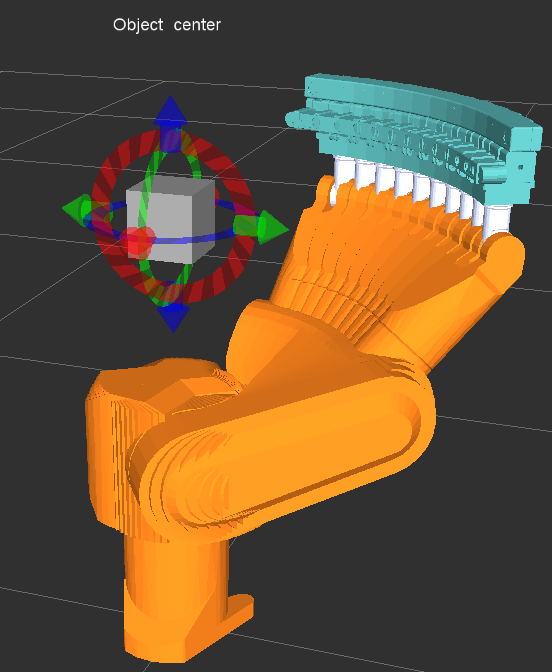
\includegraphics[scale=0.5,trim=0 0 0 0]{graphics/04_decisionmaking/robot_moving_around_object.png}%trim=l b r t
		\caption{The spin center is moveable by an interactive marker. The robot has planned a path to the next desired pose}
		\label{fig:robot_moving_around_object}
	\end{center}
\end{figure}

%\subsection{SMACH}
%SMACH = Next best view ready code
%state machine diagram?

\subsection{Special message type}
For easy offline manipulation of data a messagetype has been defined to carry the information acquired at each pose. Using this format allows the data to be captured at one point in time and processing at another by using rosbag between the nodes. Initially the message only contains the pose id, max number of poses and poses of the sensors, it is then passed on to the stereo camera node where the captured images are appended. Afterwards the dense\_stereo node creates and appends 3D information from the captured images and finally it can be passed to the reconstruction node.

\begin{figure}[htb]
	\begin{center}
		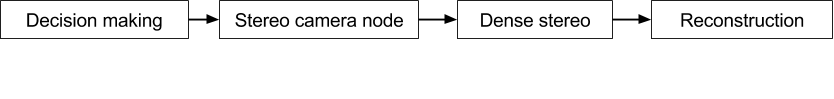
\includegraphics[scale=0.5,trim=0 50 0 0]{graphics/04_decisionmaking/message_path.png}%trim=l b r t
		\caption{The path of the message between the related nodes in the system. In each node new data is appended}
		\label{fig:message_path}
	\end{center}
\end{figure}


%Capture signal

%\subsection{Error handling}
%We do not make errors!
